\documentclass[8pt]{article}
\usepackage{amsfonts}
\usepackage{amsmath}
\usepackage{mathtools}
\usepackage{subcaption}
\usepackage{graphicx}
\usepackage{float}
\usepackage{pythonhighlight}
\usepackage[all]{foreign}
\usepackage{cleveref}
\usepackage{fmtcount}
\usepackage{verbatim}
\usepackage{multicol}
\usepackage{xparse}
\usepackage{listings}
\usepackage[inline]{enumitem}

\NewDocumentCommand\weight{}{\textsf{weight}\xspace}
\DeclareMathOperator{\arctantwo}{arctan2}

\title{Probabilistic Logic Programming Exam}
\author{
        Francesco Fabiano, Luca Geatti\\
        \footnotesize Department of Mathematics, Computer Science and Physics \\
        \footnotesize University of Udine\\
        \footnotesize via delle Scienze, 206, 33100 Udine, \underline{Italy}
}
\date{\footnotesize\today}


\begin{document}
\maketitle
\paragraph{Abstract}
This is a report for the exam of the PhD course on Probabilistic Logic
Programming, held at University of Udine in the academic year 2018-2019.



\section{Introduction}

  \paragraph{The problem}
    Modern \textit{biometrics}-based tools exploit the fact that these biometric characteristics, used for the verification of an individual’s identity, are unique from person to person.
    That is why the majority of the studies in this field aim to generate biometric tools that are able to distinguish even twins.
    
    The purpose of these researches is to identify the uniqueness of each \textit{fingerprint}, facial feature or any others biometric characteristics of a person.
    For all these reasons, to the best of our knowledge, no study exists that tries to exploit heredity in such features.
    \textit{Heredity} is usually defined as \textit{the transmission of characteristics from the parents to the offspring}
    and is commonly known that traits as body size, hair color, skin color, eye color, etc. are inherited.
    Researchers have found that the inheritance process is originated at cellular level as the cells are the unit of structures and, therefore, the units of heredity.
    %Chromosomes in all of the body cells of a single individual are alike.
    %Thus, the individual functions as a single unit—alike in every cell yet different from all other people.
    
    In this study we try to extrapolate from a fingerprint, the most used biometric characteristics, a data structure informative enough to be used for heredity-finding purposes (as explained in the following).
    This newly created data structure will be defined starting from the fingerprint \textit{minutiae}, informative points of the fingerprint itself often used for the \textquoteleft classical' biometrics-based recognition (The circles in~\cref{fig:ske_min}).
  \paragraph{Fingerprint Inheritance}\label{par:heredity}
  The main objective of this study is to reconstruct through \textit{P.L.P.} a data structure that can be used for inheritance recognition on fingerprint.
  We decided to tackle this specific problem after reading several publications that confirmed our idea that fingerprints, as most of our physical characteristics, are, in a certain sense, inherited.
  Most of these studies found connections between fingerprints of relative but not a precise pattern that could describe this property.
  Our research aims to define more formally what exactly makes two fingerprints related w.r.t. inheritance thanks to the use of
  \begin{enumerate*}[label=\roman*)]
  	\item logic programming (\textit{A.S.P.}, \textit{C.L.P.});
  	\item images classification (\textit{Convolutional Neural Networks}); and
  	\item pattern analysis.
  \end{enumerate*}
	All of these techniques need to be used on a data structure that has to be more informative that the ones already used to represent fingerprints in the modern biometric-based tools. That is why we chose the graph of the minutiae and this graph is exactly what this work aims to extrapolate from each fingerprint (often store with incomplete information).
  
  \paragraph{Exploiting P.L.P.}
    The main idea of the study, as said before, is to capture a new fingerprint description starting from the widely used minutiae.
    This new structure can be pictured as a directed \textit{graph} with some constrains on the edges: each node can have at most one \textit{incoming edge} and at most two \textit{outgoing}.
    The main idea behind this graph (shown in~\cref{fig:ske_min_graph}) is that it should \textquoteleft emulate' the \textit{skeleton} (the black lines of~\cref{fig:ske_min}) of the fingerprint.
    As reconstructing this graph could be somewhat trivial when in posses of the fingerprint's original image, it is not when the only available information are the fingerprint's minutiae.
    Unfortunately this is the case in most of the official databases where, due to space optimization, the fingerprints are only stored as a set of minutiae along with few other information.
    
   	\begin{figure}
    	\centering
    	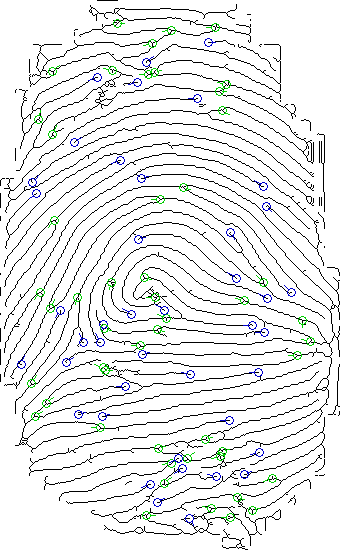
\includegraphics[width=0.35\linewidth]{img/ske_min}
    	\caption{The skeleton and the minutiae of a fingerprint.}
    	\label{fig:ske_min}
    \end{figure}
    
    \begin{figure}
    	\centering
    	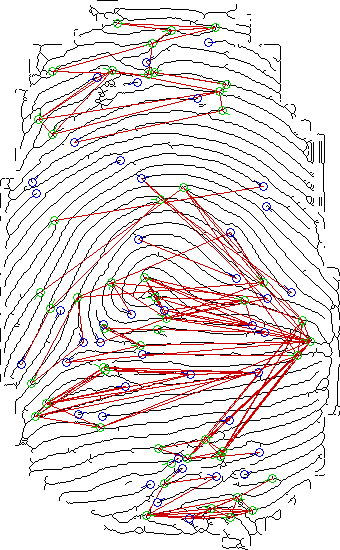
\includegraphics[width=0.35\linewidth]{img/ske_min_graph}
    	\caption{The ideal graph of the fingerprint in~\cref{fig:ske_min}.}
    	\label{fig:ske_min_graph}
    \end{figure}%
    
    This is why we decided to exploit \textit{Probabilistic Logic Programming}.
   	In fact, having all the fingerprints regular patterns
    (\cref{fig:patterns}), we could exploit these informations to reconstruct 
    the desired graph using probabilities.
   	In particular our aim is to associate each edge with a probability of existence 
    based on various factors such as: length, angle, position, crossing with other edges, 
    incoming and outgoing nodes.
   	Once that all the edges have been labeled with a probability, the result will be a 
    probabilistic graph that could be used as base for heredity-base recognition.
   	Through the use of P.L.P., it has been possible to characterize probabilistic 
    constraints that allowed this graph reconstruction.
   	As a future development, we plan to exploit the \textquoteleft learning' capabilities of 
    this paradigm, allowing the program to infer the best weight for each constraints 
    relative to each pattern.

    \begin{figure}
		\centering
		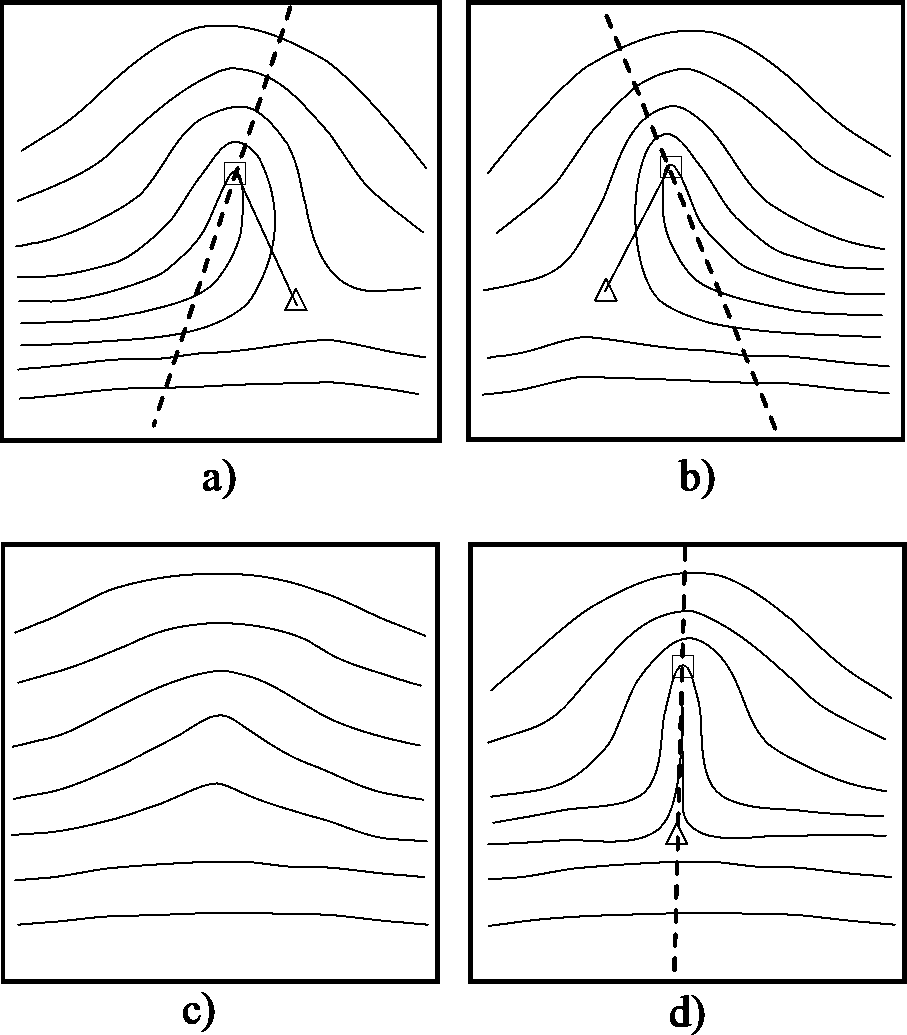
\includegraphics[width=0.6\linewidth]{img/patterns}
		\caption{Fingerprint patterns as they appear at a coarse level: a) \textit{left loop}, b) \textit{right loop}, c) \textit{\textit{arch}}, and d) tented arch; squares denote loop-type singular points, and triangles
			delta-type singular points..}
		\label{fig:patterns}
	\end{figure}%





%%%%%%%%%%%%%%%%%%%%%%%%%%%%%%%%%%%%%%%%%%%%%%%%%%%%%%%
%%% Encoding
%%%%%%%%%%%%%%%%%%%%%%%%%%%%%%%%%%%%%%%%%%%%%%%%%%%%%%%
\section{Encoding}
\label{sec:encoding}
We start by describing the basic predicates introduced to model
the problem. In order to model a minutia, we introduced the predicate
  \begin{center}
    \textsf{minutia(X,Y,D,T)}
  \end{center}
where $\textsf{X},\textsf{Y} \in \mathbb{N}$ are the coordinates\footnote{Note 
that the pixel with coordinates $(0,0)$ is the top left one.}
of the minutiae inside the image along the X-axis and Y-axis, respectively;
$\textsf{D} \in [0,2\pi]$ is the direction, expressed in radians; 
and $T \in \{e,b\}$ is the type of the fingerprint ($e$ stands for
\emph{ending}, $b$ for \emph{bifurcation}).
The second predicate is
  \begin{center}
    \textsf{type\_fingerprint(T)}
  \end{center}
where $\textsf{T}\in\{
  \textsf{tented\_archs},
  \textsf{plain\_archs},
  \textsf{left\_loop},
  \textsf{right\_loop},
  \textsf{whorl}
\}$; 
basically, it expresses which type the overall fingerprint belongs to
(see~\cref{fig:patterns}).
Finally, \textsf{max\_X(N)} and \textsf{max\_Y(N)} express the number
of pixels of the image along the X-axis and the Y-axis, respectively.
The \emph{knowledge base} of our program will be the set of all the 
\textsf{minutia/4} predicates corresponding to the input file,
the \textsf{type\_fingerprint/1} predicate and the \textsf{max\_X/1}
and \textsf{max\_Y/1} predicates. For example:
  \begin{center}
  \begin{lstlisting}[language=Prolog,frame = single,basicstyle=\footnotesize\ttfamily]
max_Y(450).
max_X(338).
type_fingerprint(tented_archs).
minutia(338,84,3.14888994760949725,e).
minutia(47,450,0.1334635904729058,e).
minutia(39,302,0.8478169733934057,e).
...
minutia(58,256,5.31793364398966,b).
minutia(94,104,0.09966865249116204,b).
minutia(62,272,5.135242906517631,b).
  \end{lstlisting}
  \end{center}
Since what we want to retrieve are the edges between the minutiae along
with their probability of existence, we introduced the predicate
  \begin{center}
    \textsf{edge($X_1,Y_1,X_2,Y_2$)}
  \end{center}
where $(X_1,Y_1)$ are the coordinates of one end and $(X_2,Y_2)$
the coordinate of the other end.
Since in our setting we want undirected edges (their direction does not
matter), some simmetry breaking constraints can be added to the 
encoding, aiming at removing specular but equivalent solutions; in
particular, we constrained that there must exists only left-to-right
edges.

\subsection{Structure constraints}\label{sub:structure_cons}
We introduce two structure constraints to forbid wrong edges
in the final solution.
\begin{itemize}
  \item
    each B-minutia has exactly $3$ incident edges. This has been achieved
    using the \texttt{aggregate\_all} predicate, as follows:
      \begin{lstlisting}[language=Prolog,frame = single,basicstyle=\footnotesize\ttfamily]
b_inc_edge :-  aggregate_all(count, edge(X,Y,X1,Y1), Count1),
               aggregate_all(count, edge(X2,Y2,X,Y), Count2),
               Sum is Count1+Count2, Sum == 3,
               minutia(X,Y,_,b),
               minutia(X1,Y1,_,_),
               minutia(X2,Y2,_,_).
      \end{lstlisting}
  \item
    similarly, each E-minutia has exactly $2$ incident edges.
\end{itemize}
With the rule \texttt{valid\_graph :- b\_inc\_edge, e\_inc\_edge} we impose
these two structure constraints.

\section{Probability constraints}
\subsection{Tented and Plain Archs}
%\paragraph{Contraint POS1}:
%Given two E-minutiae belonging to a tented arch fingerprint, we note that 
%the probability of existence of an edge between these two minutiae 
%is high if they have opposite directions and low if the have 
%the same direction.
%Let $M_1=(X_1,Y_1,D_1,e)$ and $M_2=(X_2,Y_2,D_2,e)$ be two E-minutiae.
%Let 
%  \begin{align*}
%    \weight_d(M_1,M_2) \coloneqq 
%    \frac{
%      \left( \pi - \Big\lvert \lvert D_1-D_2 \rvert - 
%      \pi \rvert\Big\rvert \right)}{\pi}
%  \end{align*} 
%The more $\lvert D_1-D_2 \rvert$ is close to $\pi$ (resp. $0$), the more 
%$weight_d(M_1,M_2)$ is close to $1$ (resp. $0$).
%With Constraint TA1, we give the value $weight_d(M_1,M_2)$ to the probability 
%of existence of an edge between $M_1$ and $M_2$.
%
%\paragraph{Contraint POS2}:
%Given two B-minutiae belonging to a tented arch fingerprint, the more
%these two minutiae are distant (either in the x-axis or in the y-axis)
%the less an edge between them is likely to exists.
%
%Let $M_1=(X_1,Y_1,D_1,b)$ and $M_2=(X_2,Y_2,D_2,b)$ be two B-minutiae.
%Let $max_x$ and $max_y$ be the maximum value for the x-coordinate and
%y-coordinate, respectively. We define:
%  \begin{align*}
%    \weight_x(M_1,M_2) \coloneqq
%    \frac{\lvert X_1 - X_2 \rvert}{max_x}
%  \end{align*}
%  \begin{align*}
%    \weight_y(M_1,M_2) \coloneqq
%    \frac{\lvert Y_1 - Y_2 \rvert}{max_y}
%  \end{align*}
%We give the value $\weight_x$ and $\weight_y$ to the probability 
%of existence of an edge between $M_1$ and $M_2$.
In this part, we describe probability rules for the tented and plain archs 
fingerprints: you can refer to fig. 3c, fig. 3d or to~\cref{fig:arch} as examples.

\paragraph{Constraint POS}
In this paragraph, we give a constraint for the edges inside a tented
or plaing arch fingerprint that link the \emph{direction} of the two
minutiae with the probability of existence of an edge between them.
Given two minutiae $M_1$ and $M_2$ (of any kind) beloning to a tented 
or plain arch fingerprint,
we note that the probability of existence of an edge between these two
respects this rule: the more the directions of both the minutiae
is close to the straight line connecting $M_1$ and $M_2$ the more the
probability is high (the red lines in~\cref{fig:arch}).
Let $M_1=(X_1,Y_1,D_1,\_)$ and $M_2=(X_2,Y_2,D_2,\_)$ be two minutiae.
Let $\alpha_1=\arctantwo(Y1-Y2,X1-X2)$ and $\alpha_2=\arctantwo(Y2-Y1,X2-X1)$:
$\alpha_1$ (resp. $\alpha_2$) measures the value of the angle (in randians) between 
the direction of $M_1$ (resp. $M_2$) and the straight line between $M_1$ and
$M_2$.
We define:
  \begin{align*}
    \weight_{POS} \coloneqq
    W \cdot (1-\frac{\lvert D1-\alpha_1\rvert+\lvert D2-\alpha_2\rvert}{2\pi})
  \end{align*}
where in the case of tented archs $W=1$: in the following we will explain the
meaning of variable $W$.
With Constraint POS, we give the value $weight_{POS}(M_1,M_2)$ to the probability 
of existence of an edge between $M_1$ and $M_2$.

\paragraph{Distance Constraints}
In this paragraph, we give a total of three constraints for edges inside
a tented or plain archs fingerprint that take into consideration the
\emph{distance} between two minutiae.
Let $M_1=(X_1,Y_1,D_1,\_)$ and $M_2=(X_2,Y_2,D_2,\_)$ be two minutiae.
  \begin{itemize}
    \item \textbf{DIST\_ARCH\_1}: the more the position of $M_1$ and $M_2$
          on the Y-axis is similar, the more an edge between $M_1$ and $M_2$
          is likely to exist. We assign $\weight_{DA1}$ to the probability
          of existence of this edge, where:
            \begin{align*}
              \weight_{DA1} \coloneqq 1-\frac{\lvert Y1-Y2\rvert}{max\_Y}
            \end{align*}
    \item \textbf{DIST\_ARCH\_2}: the same as the previous point, but with
          the X-axis;
    \item \textbf{DIST\_ARCH\_3}: the more the X-coordinate of the midpoint of 
          the line between $M_1$ and $M_2$ is close to the half of the image,
          the more this edge is likely to exist. In other words, we want that
          minutiae that are \emph{not balanced} w.r.t. to the center of the
          image (\eg one minuties close to the center but the other on the 
          extreme right) are unlikely. We assign $\weight_{DA3}$ to the 
          probability of existence of this edge, where:
            \begin{align*}
              \weight_{DA3} \coloneqq 1 -
              \frac{\lvert \frac{\lvert X1-X2 \rvert}{2} - \frac{max\_X}{2}
              \rvert}{max\_X}
            \end{align*}
  \end{itemize}


\subsection{Left and Right Loop}
%Non dividiamo in 4 quadranti, ma piuttosto diamo un peso a tutte le
%regole, cioè sia a quelle standard dei plain archs (due quadranti superiori)
%sia a quelle specifiche per i left/right loops (due quadranti inferiori).
%
%I pesi per le probabilità sono opposti per i due tipi di regole, a seconda
%che si avvicinino o meno alla parte bassa o alta dell'immagine. L'idea è
%questa:
%  \begin{itemize}
%    \item
%      piu mi avvicino alla parte bassa dell'immagine e piu do peso alle
%      regole per i left/right loops. Faccio questo \emph{moltiplicando}
%      la probabilita dell'arco per il valore:
%        \begin{align*}
%          1 - Y_1 \cdot Y_2
%        \end{align*}
%    \item
%      similmente, piu mi avvicino alla parte alta dell'immagine e piu 
%      do peso alle regole per i plain archs.
%  \end{itemize}
In this part, we describe the probability rules for the left and right loop
fingerprints: you can refer to fig. 3a, fig. 3b or to~\cref{fig:loop} as examples.
Since, in their upper region, left and right loop fingerprints exhibit a behavior similar
to that of tented and plain archs fingerprints, we decided to use the
contraints we described above in these cases as well. In particular, we
note that in the upper region, the behavior of a left or right fingerprint is
very similar to that of a plain of tented arch. For this reason, we
parameterized \emph{Constraint POS} with the variable $W$:
  \begin{itemize}
    \item
      if we have a tented or plain archs fingerprint, then $W$ is $1$, meaning
      that the rule has the same weight for all the points in the image;
    \item
      otherwise, in the case of left or right loop fingerprint, $W$ is
      computed by the predicate $weight\_rule(W,Y1,Y2)$, which assigns 
      $W$ the value:
        \begin{align*}
          W \coloneqq 
          \lvert 1-\frac{Y1}{max_Y} \rvert 
          \cdot 
          \lvert 1-\frac{Y2}{max_Y} \rvert
        \end{align*}
      Therefore, the closer the two points are to the upper region of a
      left or right loop fingerprint, the more we give weight to \emph{Constraint POS}.
  \end{itemize}

\paragraph{Constraint LOOP}
Given a left or right loop fingerprint, we noted that the ending-type
minutiae located in the \emph{lower region} of the image are clustered along
a vertical line as shown in Figure~\cref{fig:loop}.  
This behavior is captured by \emph{Constraint LOOP}, which gives to
the edge between two minutiae $M_1$ and $M_2$ belonging to a left or right loop
the probability $\weight_{LOOP}$, where:
  \begin{align*}
    \weight_{LOOP} \coloneqq
    (1-W)\cdot 
    (1-\frac{\lvert X1-X2 \rvert}{max\_X})
  \end{align*}
Again, $(1-W)$ models the fact that the more the two minutiae are lower in 
the image, the more weight we want to give to the rule.  



\paragraph{Constraints LL and LR}
Along the above-mentioned line on which the minutiae of a left or right loop
fingerprint are located, we indentified another constraint: minutiae have to
be \emph{balanced} along this line, in a very similar way we did for
\emph{DIST\_ARCH\_3}. In other words, the more the midpoint of the straight line 
between two minutiae is closer to the \emph{third quartile}\footnote{For third
quartile, we wean the set of points $(X,Y)$ such that $Y=\frac{3}{4}\cdot
max\_Y$} of the image, the more an edge between them is likely.

Overall, the probability given by \emph{Constraint LL} to the existence of
an edge is $\weight_{LL}$, where:
  \begin{itemize}
    \item
      $\weight_{LL}^\prime \coloneqq 
        (1-W) \cdot (1-\frac{X1}{max\_X}) \cdot (1-\frac{X2}{max\_X})$ 
    \item
      $\weight_{LL} \coloneqq
        \weight_{LL}^\prime \cdot (1-
        \frac{\lvert \frac{\lvert Y1-Y2 \rvert}{2} - \frac{3}{4}\cdot max\_Y
        \rvert}{max\_Y})$
  \end{itemize}
Recall that the more $(1-W)$ is high, the more we are in the lower region
of the image. In the same way, the more we are in the bottom left region of the
image, the more $\weight_{LL}^\prime$ is high. 
Finally, with $\weight_{LL}$ we are saying that the more the points are 
\emph{balanced} w.r.t. the third quartile, the more an edge between them
is likely to exist.

\emph{Constrain RL} does the same expect that $\weight_{RL}^\prime$ is
defined as follows:
  \begin{align*}
    \weight_{RL}^\prime \coloneqq 
      (1-W)\cdot \frac{X1}{max\_X} \cdot \frac{X2}{max\_X}
  \end{align*}
in order to give more weight to the points in the bottom right region.
\begin{figure}
	\centering
   	\begin{subfigure}{.48\textwidth}
   			\centering
	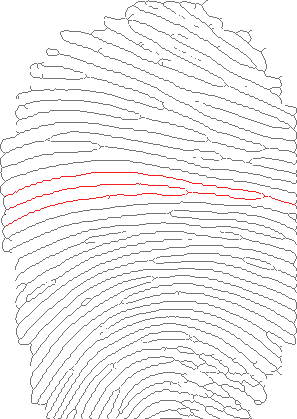
\includegraphics[width=0.9\linewidth]{img/arch}
	\caption{Skeleton of an \textit{arch} type. In red are highlighted examples of the describe ridges.}
	\label{fig:arch}
\end{subfigure}%
\hfill
\begin{subfigure}{.48\textwidth}
	\centering
	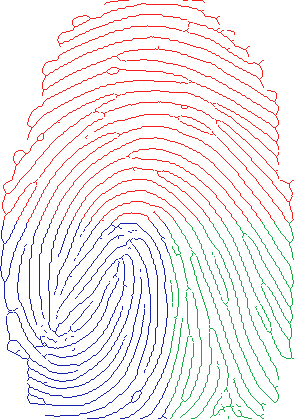
\includegraphics[width=0.86\linewidth]{img/loop}
	\caption{Skeleton of an \textit{left-loop} type. In blue the quadrant that encapsulates the loop while in red and green the parts captured by the arch constraints.}
	\label{fig:loop}
\end{subfigure}%
\caption{Example of the properties captured by our constraints.}
\label{fig:example}
\end{figure}

\section{Computation of the graph}
With the query 
  \begin{center}
  \begin{lstlisting}[language=Prolog,frame = single,basicstyle=\footnotesize\ttfamily]
findall([X1,Y1,X2,Y2,P],prob(edge(X1,Y1,X2,Y2),P),Results).
  \end{lstlisting}
  \end{center}
we can retrieve all the results of the unification of \texttt{edge(X1,Y1,X2,Y2)}
with the logic program's rules. The result is a list of this type:
  \begin{center}
  \begin{lstlisting}[language=Prolog,frame = single,basicstyle=\footnotesize\ttfamily]
Results = [
  [39, 302, 58, 256, 0.8761637920914388],
  [39, 302, 338, 84, 0.9757900620331998],
  [39, 302, 62, 272, 0.921175664640193],
  [39, 302, 47, 450, 0.901470217393874],
  ...
  [47, 450, 338, 84, 0.9445871662832741],
  [94, 104, 338, 84, 0.9562089492578153]
]
  \end{lstlisting}
  \end{center}
Each tuple in the list is an edge labeled with its probability of existence,
based on the rules we described above. This is \emph{not} the final graph
we want to retrieve, since it is just the collection of all the results
of the unification. Thus, we propose the following procedure:
  \begin{enumerate}
    \item
      from the result of the \texttt{findall} query, take the tuple
      \texttt{[X1,Y1,X2,Y2,P]} with the highest probability \texttt{P};
    \item
      add the corresponing edge to the knowledge base, \ie
      add \texttt{edge(X1,Y1,X2,Y2)} to the program;
    \item
      execute again the \texttt{findall} query
      \begin{enumerate}
        \item
          if the result is empty, then it means that the edge we just
          added violates some structure constraints (see
          \cref{sub:structure_cons}); thus, we delete it from the knowledge
          base and from the result of the latest \texttt{findall} query, and we
          go back to Point 1; 
        \item
          otherwise, we can just go back to Point 1 and reiterate the process.
      \end{enumerate}
  \end{enumerate}
\paragraph{Termination condition:} once all the edge inside
the latest \texttt{findall}'s list are no-good, \ie once this list becomes empty,
then we stop the algorithm: the knowledge base contains the graph for the
fingerprint.

\section{Conclusions}
During this work we studied and tackled the problem of reconstructing the skeleton 
of a fingerprint only using the available information on the official databases, 
\ie the \emph{minutiae}.
As already said we are exploiting probabilistic logic programming to reconstruct the 
\textquotedblleft most probable skeleton".
Thanks to our script (the file named \textquotedblleft \textit{fingerprints.pl}") it 
is possible to extract the list of edges with relative probability. 
Then with a simple iterative process on the script it would be possible to retrieve 
the whole graph.
%: at every iteration we add the most probable edge found at the previous 
%iteration to the \textquotedblleft bad\_edges" so we can find the new most probable edge.

As we can see in~\cref{fig:concl} the graph generated through our tool is somewhat similar 
to the one that has been extrapolated from the binary image itself.
An important factor to keep in mind is that the image obtained by out \textit{P.L.P.} procedure~\cref{fig:concl-plp}, even if it differs from the original one~\cref{fig:concl-c}, follows accurately what we formalized.
This means that the \textit{P.L.P.} script needs only refinements in the constraints to produce results that can be representative of real fingerprint.
That is why, even if the two graphs obviously differ, the results are promising and this tool is certainly 
to keep in mind for future studies on inheritance on fingerprints.

\begin{figure}
	\centering
	\begin{subfigure}{.48\textwidth}
		\centering
		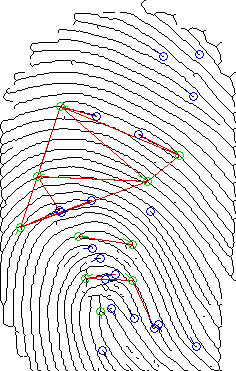
\includegraphics[width=0.9\linewidth]{img/c-final}
		\caption{Graph obtained from the original binary image.}
					\label{fig:concl-c}
	\end{subfigure}%
	\hfill
	\begin{subfigure}{.48\textwidth}
		\centering
		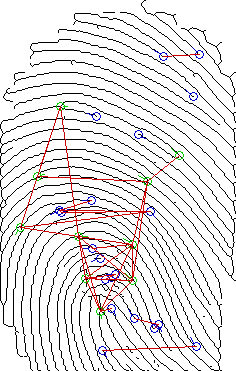
\includegraphics[width=0.86\linewidth]{img/plp-final}
		\caption{Graph obtained from our script.}
			\label{fig:concl-plp}
	\end{subfigure}%
	\caption{Graphs confrontation.}
	\label{fig:concl}
\end{figure}

As future works we plan to:
\begin{itemize}
	\item Increase the precision of our tool by introducing more constraints for each 
        type of fingerprint.
	\item Automatize the iterative procedure to permit an easier use of the tool. 
        In particular we aim to formalize directly in the \textit{P.L.P.} file the printing 
        of the whole graph.
	\item As we have a large set of fingerprints images ($\approx 3\ 000$) we think that 
        exploiting the learning component of \textit{cplint} could bring really promising results.
\end{itemize}






\end{document}
